\chapter{Transforming Your Core Services}


\section{Introduction}

As an IT consultant, your ability to efficiently gather requirements, prototype solutions, and present data can set you apart from the competition. In this chapter, we'll explore how to leverage no-code tools to revolutionize these core services, making your consulting practice more efficient and effective.


\section{Automating Requirements Gathering}

One of the most time-consuming aspects of IT consulting is gathering and documenting client requirements. Let's explore how we can streamline this process using our no-code toolkit.

\subsection{The Traditional vs. Automated Approach}

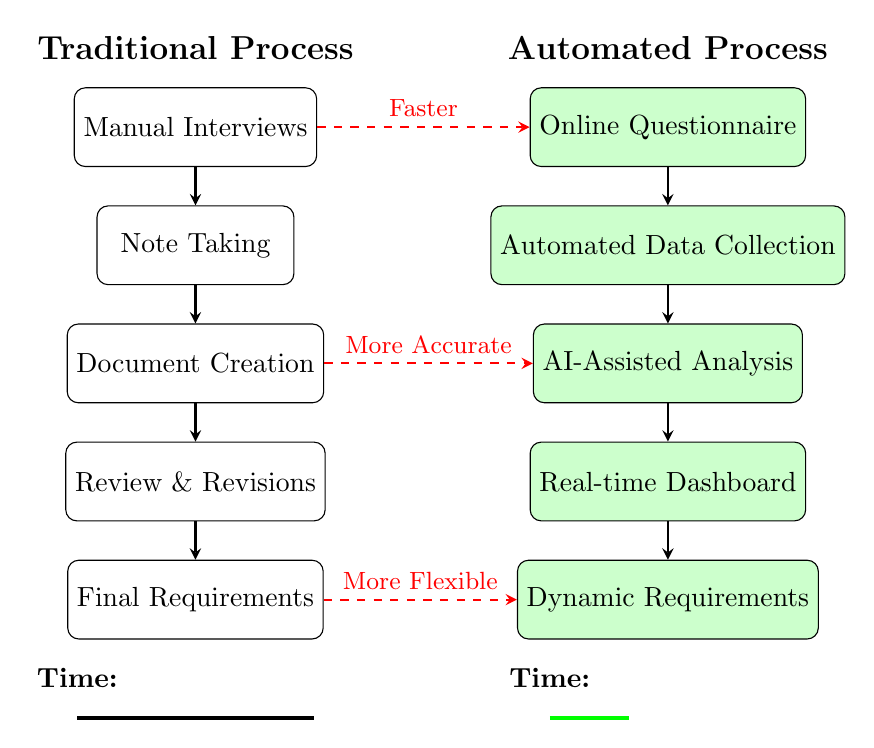
\begin{tikzpicture}
    [
    box/.style={draw, rounded corners, minimum width=2.5cm, minimum height=1cm, align=center},
    arrow/.style={->, >=stealth, thick},
    title/.style={font=\bfseries\large},
    subtitle/.style={font=\bfseries}
    ]

% Traditional Process
    \node[title] at (-3, 4) {Traditional Process};
    \node[box] (t1) at (-3, 3) {Manual Interviews};
    \node[box] (t2) at (-3, 1.5) {Note Taking};
    \node[box] (t3) at (-3, 0) {Document Creation};
    \node[box] (t4) at (-3, -1.5) {Review \& Revisions};
    \node[box] (t5) at (-3, -3) {Final Requirements};

    \draw[arrow] (t1) -- (t2);
    \draw[arrow] (t2) -- (t3);
    \draw[arrow] (t3) -- (t4);
    \draw[arrow] (t4) -- (t5);

% Automated Process
    \node[title] at (3, 4) {Automated Process};
    \node[box, fill=green!20] (a1) at (3, 3) {Online Questionnaire};
    \node[box, fill=green!20] (a2) at (3, 1.5) {Automated Data Collection};
    \node[box, fill=green!20] (a3) at (3, 0) {AI-Assisted Analysis};
    \node[box, fill=green!20] (a4) at (3, -1.5) {Real-time Dashboard};
    \node[box, fill=green!20] (a5) at (3, -3) {Dynamic Requirements};

    \draw[arrow] (a1) -- (a2);
    \draw[arrow] (a2) -- (a3);
    \draw[arrow] (a3) -- (a4);
    \draw[arrow] (a4) -- (a5);

% Comparison arrows
    \draw[arrow, dashed, red] (t1) -- node[above, sloped, text=red] {\small Faster} (a1);
    \draw[arrow, dashed, red] (t3) -- node[above, sloped, text=red] {\small More Accurate} (a3);
    \draw[arrow, dashed, red] (t5) -- node[above, sloped, text=red] {\small More Flexible} (a5);

% Time comparison
    \node[subtitle] at (-4.5, -4) {Time:};
    \draw[ultra thick] (-4.5, -4.5) -- (-1.5, -4.5);
    \node[subtitle] at (1.5, -4) {Time:};
    \draw[ultra thick, green] (1.5, -4.5) -- (2.5, -4.5);

\end{tikzpicture}

\subsection{Setting Up an Automated Requirements Workflow}

Let's create a comprehensive requirements gathering system using n8n, NoCoDB, and BudiBase:

1. \textbf{Initial Questionnaire}: Use n8n to create a webhook that receives responses from a Google Form.

% TODO @screenshot: n8n webhook node configuration for receiving Google Form responses

2. \textbf{Data Storage}: Configure NoCoDB to store and categorize the received requirements.

% TODO @screenshot: NoCoDB table structure for storing requirements

3. \textbf{Stakeholder Notifications}: Set up a n8n workflow to notify relevant team members about new requirements.

% TODO @screenshot: n8n workflow for stakeholder notifications

4. \textbf{Requirements Dashboard}: Create a BudiBase app to visualize and manage requirements.

% TODO @screenshot: BudiBase requirements dashboard

5. \textbf{Automated Follow-ups}: Use n8n to schedule and send follow-up questions based on initial responses.

% TODO @screenshot: n8n workflow for automated follow-up emails

\subsection{Implementing the Triplet Questioning Technique}

The Triplet Questioning technique is a powerful method for eliciting detailed requirements. Let's automate this process:

1. Set up a series of n8n workflows to ask the three key questions:
- "What is your requirement?"
- "What does that give you of value?"
- "Which value is most important?"

2. Use NoCoDB to store and analyze the responses.

3. Create a BudiBase app for stakeholders to review and prioritize the gathered requirements.

\begin{figure}
    \centering
    \includegraphics[width=0.40\textwidth]{./figures/03-flowchart-triplet-questioning.png}
    \caption{Flowchart of the automated Triplet Questioning process}
    \label{fig:triplet-questioning}
\end{figure}


\section{Rapid Prototyping Techniques That Wow Clients}

Once you've gathered requirements, the next step is creating a prototype to validate ideas and get client feedback. No-code tools excel at rapid prototyping, allowing you to create impressive demos quickly.

\subsection{Using BudiBase for Quick UI Prototypes}

1. Create a basic dashboard layout in BudiBase.

% TODO @screenshot: BudiBase dashboard layout creation

2. Add dynamic components that pull data from NoCoDB.

% TODO @screenshot: BudiBase component linked to NoCoDB data

3. Implement user interactions and navigation.

% TODO @screenshot: BudiBase app with multiple screens and navigation

\subsection{Creating Interactive Workflows with n8n}

1. Set up an n8n workflow that simulates backend processes.

% TODO @screenshot: n8n workflow simulating a business process

2. Connect the n8n workflow to your BudiBase prototype.

% TODO @screenshot: n8n HTTP Request node configured to interact with BudiBase

3. Create a "wizard" interface in BudiBase that guides users through a process, with each step triggering actions in n8n.

% TODO @screenshot: BudiBase wizard interface connected to n8n workflow

\subsection{Prototype Presentation Best Practices}

1. Use screen recording tools to create short demo videos of your prototype in action.

2. Prepare a slide deck that outlines the problem, solution, and benefits.

3. Set up a live environment where clients can interact with the prototype themselves.

\begin{tikzpicture}
    [
    note/.style={draw, fill=yellow!20, rounded corners, text width=3cm, align=center, font=\small},
    icon/.style={font=\Large},
    arrow/.style={->, >=stealth, thick},
    title/.style={font=\bfseries\large},
    subtitle/.style={font=\bfseries}
    ]

% Title
    \node[title] at (0, 4) {Prototype Presentation Best Practices};

% Central icon
    \node[icon] (center) at (0, 0) {\faLightbulb};

% Best practices
    \node[note] (demo) at (-4, 2) {Create short demo videos};
    \node[icon] at (-5, 2) {\faVideo};

    \node[note] (deck) at (0, 3) {Prepare a concise slide deck};
    \node[icon] at (-1, 3) {\faFile};

    \node[note] (live) at (4, 2) {Set up a live interactive environment};
    \node[icon] at (5, 2) {\faLaptop};

    \node[note] (focus) at (-4, -2) {Focus on solving client problems};
    \node[icon] at (-5, -2) {\faSearchDollar};

    \node[note] (feedback) at (0, -3) {Gather real-time feedback};
    \node[icon] at (-1, -3) {\faComments};

    \node[note] (story) at (4, -2) {Tell a compelling story};
    \node[icon] at (5, -2) {\faBook};

% Connecting arrows
    \foreach \i in {demo, deck, live, focus, feedback, story}
    \draw[arrow] (center) -- (\i);

% Additional tips
    \node[note, text width=5cm] at (-6, 0) {Keep it simple:\\Focus on core features\\and main user flows};
    \node[note, text width=5cm] at (6, 0) {Be prepared:\\Anticipate questions\\and have backup plans};

\end{tikzpicture}


\section{Dynamic Data Visualization and Reporting}

Presenting data effectively is crucial for demonstrating the value of your solutions. Let's explore how to create dynamic, interactive reports using our no-code toolkit.

\subsection{Building Interactive Dashboards with BudiBase}

1. Connect BudiBase to your client's data sources (or NoCoDB).

2. Create charts, graphs, and KPI displays.

% TODO @screenshot: BudiBase dashboard with various data visualizations

3. Implement filters and date range selectors for user interactivity.

% TODO @screenshot: BudiBase dashboard with interactive filters

\subsection{Automated Report Generation with n8n}

1. Set up an n8n workflow to pull data from various sources.

2. Use n8n nodes to process and format the data.

3. Generate PDF reports using the n8n PDF creation nodes.

4. Automatically email reports to stakeholders on a schedule.

\begin{figure}
    \centering
    \includegraphics[width=0.6\textwidth]{./figures/automated_report_generation_flowchart.png}
    \caption{Flowchart of the automated report generation process}
    \label{fig:automated-report-generation}
\end{figure}

\subsection{Creating a Self-Service Reporting Tool}

Combine BudiBase and n8n to create a tool that allows clients to generate their own reports:

1. Build a BudiBase interface for report configuration.

2. Use n8n to process report requests and generate reports based on user input.

3. Deliver the generated reports back to the BudiBase interface for download.

% TODO @screenshot: BudiBase interface for custom report generation


\section{Case Study: Transforming a Traditional IT Consultancy}

Let's look at how implementing these automated processes transformed a traditional IT consultancy:

\begin{itemize}
    \item Requirements gathering time reduced by 60%
    \item Prototype delivery time cut from weeks to days
    \item Client satisfaction scores increased by 35%
    \item Consultants able to handle 3x more projects simultaneously
\end{itemize}

% @illustrate: Before and after infographic showing the transformation metrics
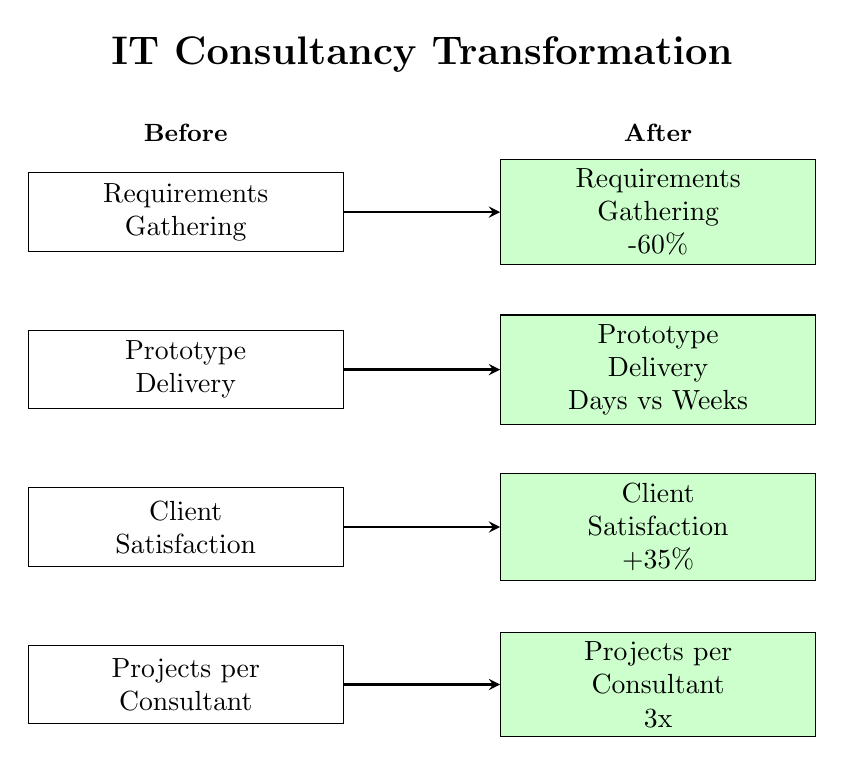
\begin{tikzpicture}
    [
    box/.style={draw, rectangle, minimum width=4cm, minimum height=1cm, align=center},
    arrow/.style={->, >=stealth, thick},
    label/.style={font=\small\bfseries}
    ]

% Before column
    \node[label] at (-3, 3) {Before};
    \node[box] (b1) at (-3, 2) {Requirements\\Gathering};
    \node[box] (b2) at (-3, 0) {Prototype\\Delivery};
    \node[box] (b3) at (-3, -2) {Client\\Satisfaction};
    \node[box] (b4) at (-3, -4) {Projects per\\Consultant};

% After column
    \node[label] at (3, 3) {After};
    \node[box, fill=green!20] (a1) at (3, 2) {Requirements\\Gathering\\-60\%};
    \node[box, fill=green!20] (a2) at (3, 0) {Prototype\\Delivery\\Days vs Weeks};
    \node[box, fill=green!20] (a3) at (3, -2) {Client\\Satisfaction\\+35\%};
    \node[box, fill=green!20] (a4) at (3, -4) {Projects per\\Consultant\\3x};

% Arrows
    \draw[arrow] (b1) -- (a1);
    \draw[arrow] (b2) -- (a2);
    \draw[arrow] (b3) -- (a3);
    \draw[arrow] (b4) -- (a4);

% Title
    \node[font=\Large\bfseries] at (0, 4) {IT Consultancy Transformation};

\end{tikzpicture}


\section{Overcoming Common Challenges}

\begin{itemize}
    \item Resistance to change from team members
    \item Integrating new processes with existing systems
    \item Ensuring data accuracy across multiple tools
    \item Maintaining a personal touch in automated processes
\end{itemize}


\section{Conclusion}

By leveraging no-code tools to automate requirements gathering, streamline prototyping, and create dynamic dashboards, you can transform your core IT consulting services. These techniques not only save you time but also impress clients with your efficiency and professionalism.

In the next chapter, we'll explore how to scale your practice using these automated solutions, allowing you to take on more clients without proportionally increasing your workload.

\textbf{Action Item}: Take one of your current projects and implement the automated requirements gathering workflow we discussed. Note how it impacts your efficiency and client satisfaction.

% TODO @qr: QR code linking to a downloadable template for the automated requirements gathering workflow